\documentclass[12pt]{article}
\usepackage{amssymb}
\usepackage{amsmath}
\usepackage{tikz}


\begin{document}

\title{Trying to converge to an equilibrium flow}
\maketitle

Throughout, Vickrey queuing model is used.

\section*{Iterative Model}

TBD

$$ h_P^{(i+1)}(\theta) = \left(1 - \alpha( d_P^{(i)}(\theta)) \right) \cdot h_P^{i}(\theta) + \frac{ \mathbb{I}_{ \{d_P^{(i)} < \varepsilon \}} (\theta) }{\sum_{P'} \mathbb{I}_{ \{d_{P'}^{(i)} < \varepsilon \}} (\theta)} \cdot \left( \sum_{P'} \alpha( d_P^{(i)}(\theta)) \cdot h_P^{i}(\theta) \right).$$

%\sum_{} \mathbb{I}_{d_P^{i}(\theta) < \varepsilon}

\section*{Dynamic Replicator Model}

Let $\mathcal{P}$ be a collection of $s$-$t$ paths. At time $\theta$, each path $P$ receives a fraction $h_P(\theta)$ of the total inflow $u(\theta)$. We are considering the replication dynamic: 

$$ \dot{h}_P = R \cdot h_P \cdot a_P, \quad ~\forall P \in \mathcal{P}, $$
where $R > 0$ is a constant, $a_P = \phi_P - \sum_{P' \in \mathcal{P}} h_{P'} \cdot \phi_{P'}$ is advantage function based on fitness $\phi$. 

 Role of the fitness can be played by negative signed average experienced travel time of the particles:
%($\theta_l = \max( \theta - w, 0 )$)
$$ \phi^{a.t.}_P(\theta, h) = - \frac{1} {F_P^+(\theta)} \left( \int_{0}^{\theta} F_P^+(\psi) d \psi - \int_{0}^{\theta} F_P^{-} (\psi) d \psi \right) .$$
Above, $F_P^+(\cdot)$, $F_P^-(\cdot)$ denote functions of accumulated path in- and outflow.

Another option is  negative signed last available travel time:

$$ \phi^{l.t.}_P(\theta, h) = -1 \cdot \begin{cases} \theta, & 0 \leq \theta < T_P(0) \\ \theta - T_P^{-1}(\theta), & \theta \geq T_P(0) \end{cases} ,$$
 $T_P(\cdot)$ is path exit time function.
 
Finally, utilising constant predictors for queues, one can use predicted travel time: 
$$ \phi^{p.t.}_P(\theta, h) = - (\hat{T}_P(\theta) - \theta) .$$
If path $P$ has only one edge, then $ \hat{T}_P(\cdot) \equiv T_P(\cdot) $.

\subsection*{Unstable instance}

Consider simple network with two parallel edges on Figure \ref{fig:instance} and inflow $u(\theta) = 5$. Let upper edge have index $0$ and lower $1$.

\begin{figure}
	\begin{center}
		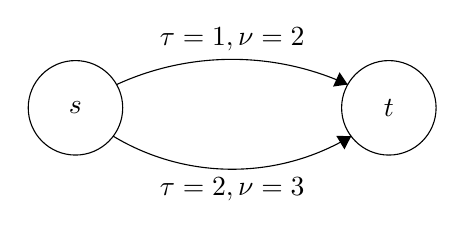
\begin{tikzpicture}[scale=0.2]
			\tikzstyle{every node}+=[inner sep=0pt]
			\draw [black] (7.2,-8.7) circle (3);
			\draw (7.2,-8.7) node {$s$};
			\draw [black] (27.1,-8.7) circle (3);
			\draw (27.1,-8.7) node {$t$};
			\draw [black] (9.808,-7.224) arc (114.62656:65.37344:17.62);
			\fill [black] (24.49,-7.22) -- (23.97,-6.44) -- (23.56,-7.35);
			\draw (17.15,-5.12) node [above] {$\tau=1, \nu=2$};
			\draw [black] (24.706,-10.5) arc (-58.92949:-121.07051:14.642);
			\fill [black] (24.71,-10.5) -- (23.76,-10.48) -- (24.28,-11.34);
			\draw (17.15,-13.1) node [below] {$\tau=2, \nu=3$};
		\end{tikzpicture}
	\end{center}
	\caption{Simple network}
	\label{fig:instance}
\end{figure}

The equilibrium flow is achieved as follows: all the inflow is redirected to the shorter edge, until both edges achieve equal costs, then the distribution is proportional to the capacities.
$$ h^*_0(\theta) = \begin{cases} 1, & 0 \leq \theta < \frac{2}{3} \\ \frac{2}{5}, &\theta \geq \frac{2}{3} \end{cases}, \quad h^*_1(\theta) = 1 - h^*_0(\theta) .$$


\subsubsection*{Numerical approximation}

Figures \ref{fig:fluctuations_avg}, \ref{fig:fluctuations_last} and \ref{fig:fluctuations_pred} show numerically computed inflow shares and fitness of replicator flow with initial condition $h_0(0) = h_1(0) = \frac{1}{2}$. The following approximation was used:

$$ h_P(\theta + \Delta\theta) \approx \frac{ h_P(\theta) \cdot e^{ R \cdot a_P \cdot \Delta \theta }} { \sum_{P'}  h_{P'}(\theta) \cdot e^{ R \cdot a_{P'} \cdot \Delta\theta } } .$$

By construction of the initial dynamic $\sum_{P'}  h_{P'}(\theta) \cdot e^{ R \cdot a_{P'} \cdot \Delta\theta } \approx 1$, but normalisation is required to remain on simplex.

\begin{center}
	\begin{figure}
	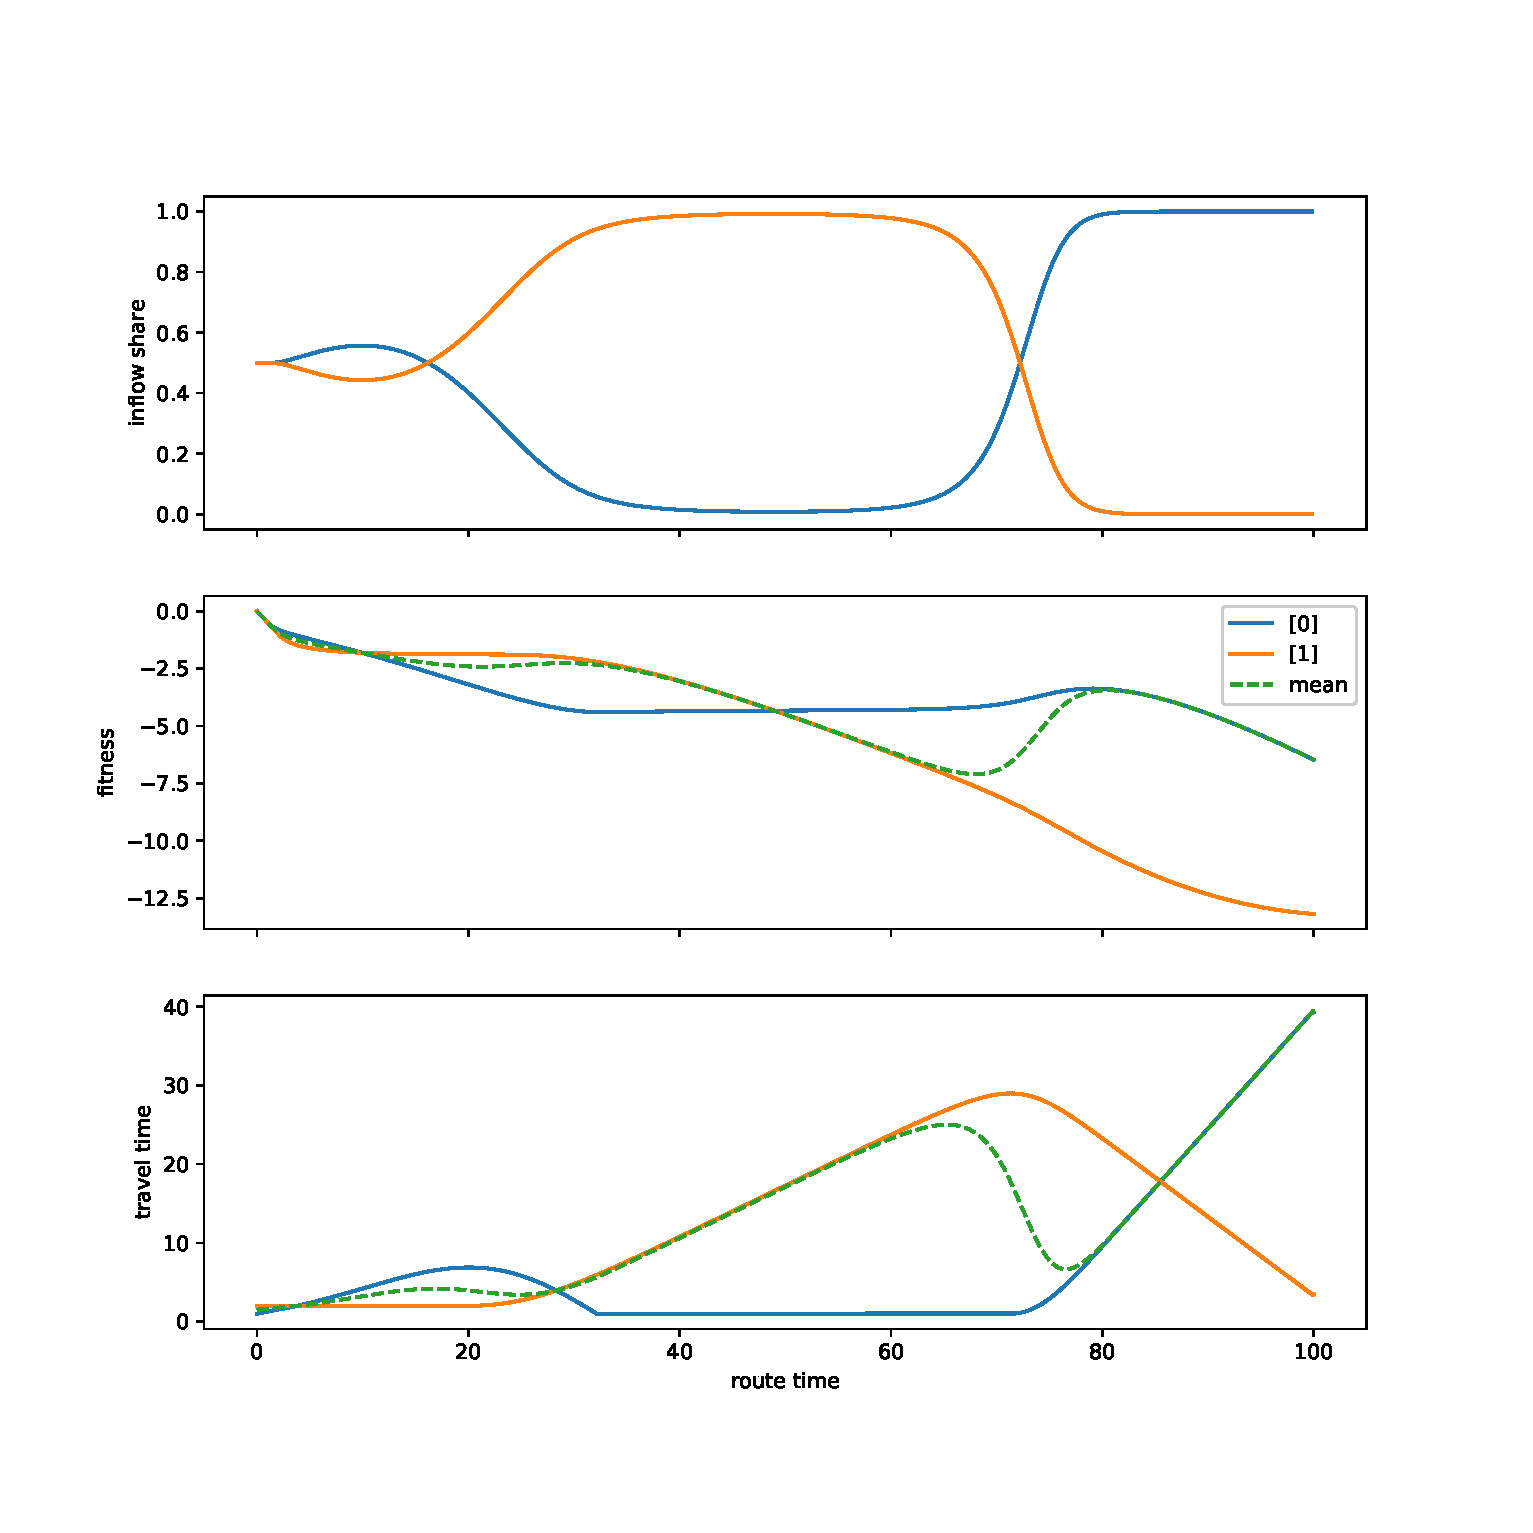
\includegraphics[scale=0.5]{img/replicator_avg_tt.eps}
	\caption{Fluctuations, average travel time }
	\label{fig:fluctuations_avg}

	\end{figure}
	
\end{center}

\begin{center}
	\begin{figure}
	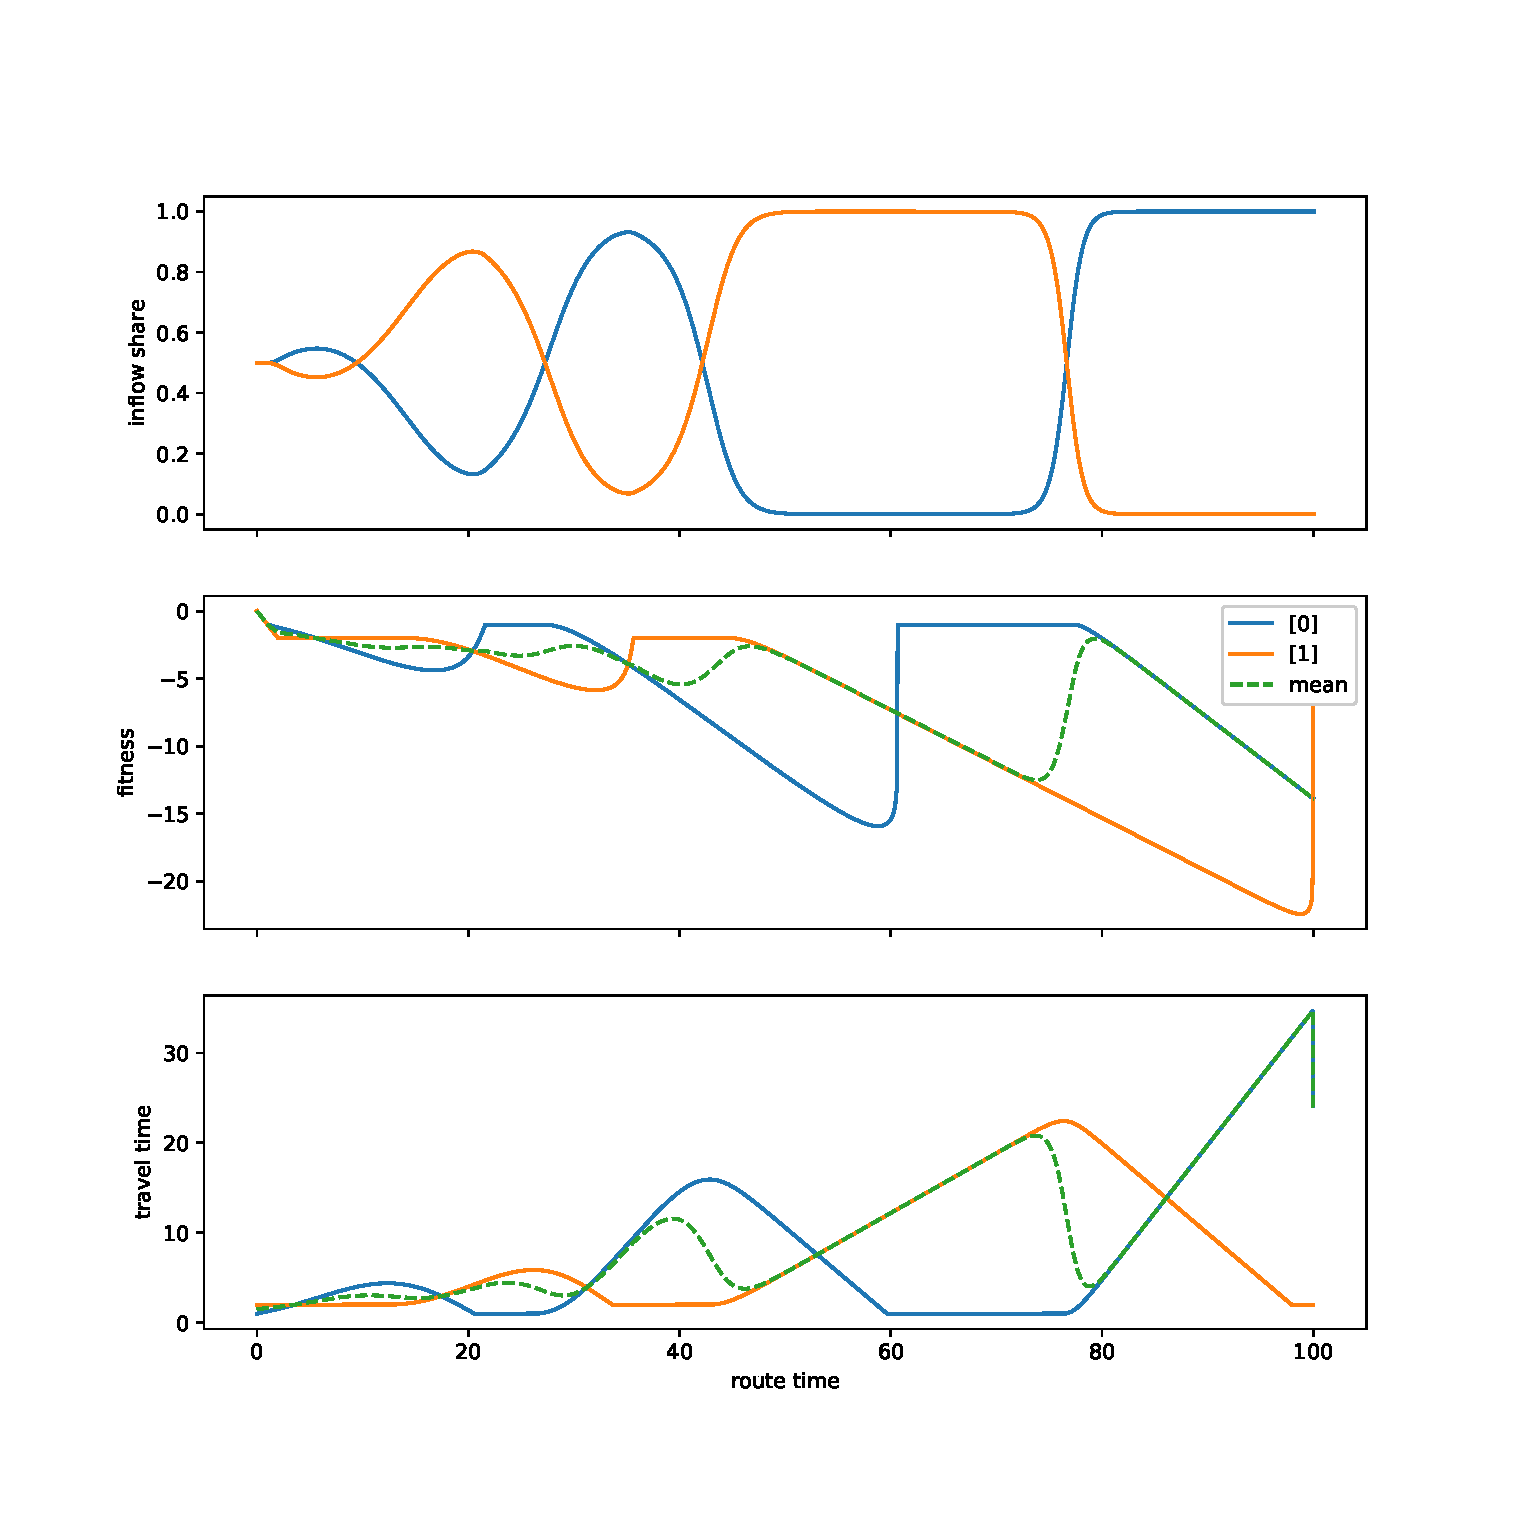
\includegraphics[scale=0.5]{img/replicator_last_tt.eps}
	\caption{Fluctuations, last travel time }
	\label{fig:fluctuations_last}

	\end{figure}
	
\end{center}

\begin{center}
	\begin{figure}
	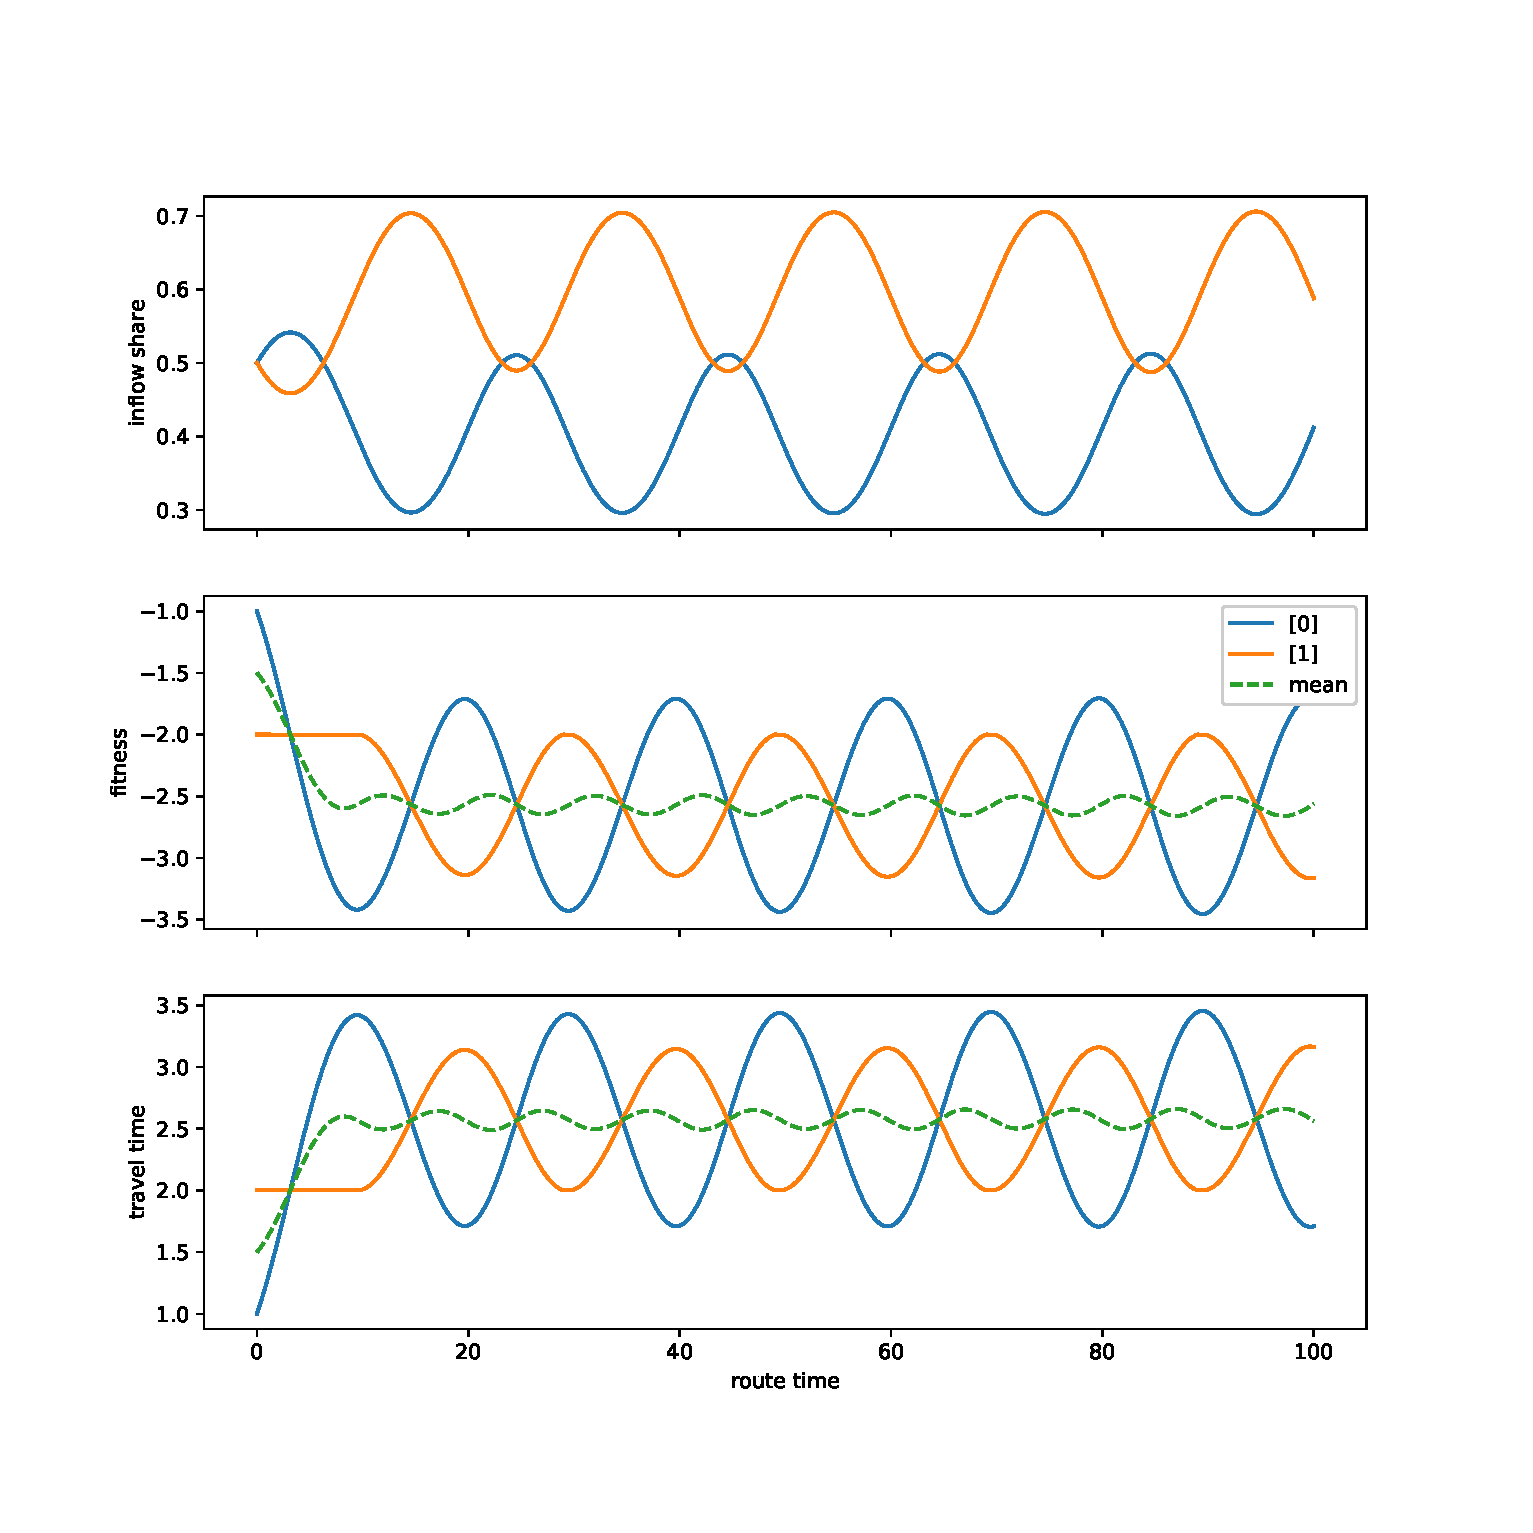
\includegraphics[scale=0.5]{img/replicator_pred_tt.eps}
	\caption{Fluctuations, predicted travel time }
	\label{fig:fluctuations_pred}

	\end{figure}
	
\end{center}

\subsubsection*{Proof ?}

Necessary condition for stability: $ \forall P: ~ \phi_P(\theta, h) = \sum_{P'} h_{P'}(\theta) \phi_{P'}(\theta, h) $. Furthermore, queues have to not change. If they do, travel times also change and equality breaks
\\
In the given example, we need inflows to equalize with edge capacities.

In cases of average travel time and last travel, influence of inflows on fitnesses is delayed for at least $\tau_0$. .
%So, stability condition can be maintained only if it was already present on the moment of last influence, and hence should have been fulfilled from the very start. 

Even when we use undelayed travel times, inflows tend to get in antiphase with fitnesses.

\end{document}